\documentclass{subfiles}
\begin{document}
%% TIME-EVOLUTION
\section{Time-evolution}\label{sec:time_evolve_methods}
In this section, we describe the numerical implementation of the time-dependent Schrödinger equation (TDSE) for evolving quantum states under a (possibly time-dependent) Hamiltonian. Our primary goal is to simulate the time evolution of a quantum wavefunction from a known initial state, using various numerical methods to approximate both the time-evolution operator and the propagation of the wavefunction itself.

We begin by discussing how to discretize time for numerical propagation. We then introduce different strategies for approximating the time-evolution operator and solving the TDSE. Several integration schemes are examined, and we compare their accuracy, stability, and efficiency. We validate our implementation using the well-known Landau-Zener model before applying the methods to the more complex double-well Morse potential system.

\subsection{Time discretization}
The foundation of any numerical time-evolution scheme lies in the discretization of the time variable. Typically, this is done by introducing a time step $\Delta t$, and defining a grid of time points $t_n = n \Delta t$ where $n$ is an integer. In general, there are two ways to do this:
\begin{itemize}
    \item \textbf{Fixed time step:} This is the most common approach, where we define a fixed time step $\Delta t$ and evolve the system in small steps. 
    \item \textbf{Adaptive time step:} This approach allows for a variable time step, where the time step is adjusted based on the dynamics of the system. This can be useful for systems with rapidly changing dynamics, where a fixed time step may not be sufficient to capture the dynamics accurately.
\end{itemize}
In this work we will be primarily employing fixed time steps, as the system we are studying is not expected to exhibit rapidly changing dynamics, due to us being in control of how we vary the potential parameters and thus perturb the system. 


\subsection{Approximating the Time-evolution operator}
In principle, the exact propagator for a quantum system is given by the time-ordered exponential of the Hamiltonian \eqref{eq:time_evolution}
\begin{align*}
    U(t, t_0) = \mathcal{T}\text{exp}\bigg(\frac{-i}{\hbar}\int_{t_0}^t H(t')dt'\bigg),
\end{align*}
or by the simpler matrix exponential $U(t) = e^{-iHt}$ for a time-independent system Hamiltonian. In either case, computing this operator exactly is impossible to evaluate analytically once our basis grows beyond a few states. Instead we must resort to numerical approximations, as discussed in section \ref{sec:time_evolution_theory} that either approximate the operator $U$ itself, or step the wavefunction forward in time. Depending on the system size and whether or not the Hamiltonian is time-dependent, different numerical techniques are more appropriate. 

For our simulations in the double-well Morse potential, we rely exclusively on two unitary-preserving, stable schemes:
\begin{itemize}
    \item \textbf{Matrix exponentiation via Padé:} This is the most straightforward approach, where we compute a direct evaluation of the matrix exponential $U=\text{exp}\big(-\frac{i}{\hbar}H\Delta t)$, typically using a Padé approximation combined with scaling and squaring, as implemented in \texttt{scipy.linalg.expm}. This method is efficient and works well for small to medium-sized matrices. Its cost scales as $\mathcal{O}(N^3)$, where $N$ is the number of basis states.
    \item \textbf{Crank-Nicolson method:} An implicit midpoint method that approximates the evolution operator as a weighted average of states at the current and next time step,
    \begin{align*}
        \psi(t + \Delta t) = \bigg(\mathbb{I} + i\frac{\Delta t H}{2}\bigg)^{-1} \bigg(\mathbb{I} - i\frac{\Delta t H}{2}\bigg) \psi(t).
    \end{align*}
    This scheme also preserves unitarity and is numerically stable, making it useful for stiff or rapidly varying systems. It is much cheaper than matrix exponentiation, with the cost equivalent to solving a single linear system at each time step.
\end{itemize}
To make an informed choice, we also test two simpler integrators purely for benchmarking purposes, and to solidify our choice of methods. These will not be applied to the full system, but rather in a controlled testbed environment on the Landau-Zener model \eqref{eq:landau_zener_model}:
\begin{itemize}
    \item \textbf{Taylor series expansion:} This method approximates the time-evolution operator as a Taylor series expansion in powers of the Hamiltonian. This is a very simple and straightforward method, but as we saw earlier, can be unstable or inaccurate unless the timestep is very small or the wavefunction norm is bounded.
    \item \textbf{Runge-Kutta methods:} These methods recast the TDSE as a first-order differential equation and integrate it stepwise. The 4th-order Runge-Kutta method (RK45) is common, though it does not preserve unitarity exactly.
\end{itemize}
By making this comparison, we shall see that the matrix exponentiation and Crank-Nicolson methods are the most reliable and efficient for our system, while the simpler methods are less accurate and more prone to numerical instabilities - even in the simple system.
%% Matrix exponentiation
\subsubsection{Matrix exponentiation}
Following the material presented in section \ref{sec:time_evolution_theory}, we know that our time-evolution operator \eqref{eq:time_evolution_operator} is given numerically, as an approximation, by the following expression \eqref{eq:numerical_time_evolution_operator}
\begin{align*}
    U(t) \approx e^{-iH(t)\Delta t} 
\end{align*}
which is easily implemented direcly in python using the \texttt{scipy.linalg.expm} function. The approximation is only valid given a small enough\footnote{Small enough is system specific} $\Delta t$, and/or slowly varying Hamiltonian. This function uses the \texttt{scipy.linalg} package to compute the matrix exponential using the algorithm introduced in \cite{Al-Mohy_Higham_2010}, which in essence in a Padé approxmation to the exponential function, using a scaling and squaring method. The \texttt{scipy.linalg.expm} function is efficient and reliable, making it well-suited for systems of moderate size. 

The function is implemented as follows:
\begin{lstlisting}[language=Python]
def time_evolution_operator(H, t, dt):
    return scipy.linalg.expm(-1j * H(t) * dt)
time = [...]
psi = [...]
psi_t = np.zeros([...])
dt = time[1] - time[0] 
for t in time:
    U = time_evolution_operator(H, t, dt)
    psi_new = np.dot(U, psi)
    psi_t.append(psi_new)
    psi = psi_new
\end{lstlisting}
where \texttt{H} is the Hamiltonian matrix, \texttt{t} is the time, and \texttt{dt} is the time step. This code snippet outlines how the \texttt{expm} function is used to compute the time-evolution operator, and how this operator is used in a time loop to evolve the wavefunction \texttt{psi}. The time-evolution operator is computed at each time step, and the wavefunction is updated accordingly. The \texttt{psi\_t} variable is used to store the wavefunction at each time step, and can be used to visualize the dynamics of the wavefunction throughout the time-evolution procedure. \\ 
While matrix exponentiation provides a robust method for computing the time-evolution operator, its accuracy for time-dependent Hamiltonians depends on how the Hamiltonian is evaluated at each time step. In particular, since $U(t, t_0) \approx \text{exp}(-iH(t)\Delta t)$, the choice of how to evaluate $H(t)$ on the interval $[t, t + \Delta t]$ can significantly affect the accuracy of the time-evolution operator. Some examples are
\begin{itemize}
    \item \textbf{Euler (explicit first order):} $U(t + \Delta t, t) = \text{exp}(-iH(t)\Delta t)$. This method is simple and fast, but inaccurate for rapidly varying Hamiltonians and/or large time steps. 
    \item \textbf{Midpoint evaluation (second order):} $U(t + \Delta t, t) = \text{exp}(-iH(t + \Delta t/2)\Delta t)$. This method is more accurate than the left-endpoint method, but still suffers from stability issues for large time steps.
    \item \textbf{Trapezoidal evaluation (second order, symmetric):} $U(t + \Delta t, t) = \text{exp}(-i(H(t) + H(t + \Delta t))/2 \Delta t)$. This method is more accurate than the midpoint method, and naturally leads into implicits methods like Crank-Nicolson. 
\end{itemize}
The choice of evaluation method depends on the specific system, and in this work, we primarily use the Euler method for simplicity and speed. \textcolor{red}{TODO: Add more details, possibly validate against the other two evaluation methods.} \\ In the next section we will discuss the different approach of using numerical integration methods to solve the time-evolution operator, namely the Crank-Nicolson method and the Runge-Kutta method. These methods are more general and can be used for time-dependent Hamiltonians, but are also more complex and computationally expensive.

\subsection{Numerical integrators}
As we have seen, direct matrix exponentiation provides a robust and unitary method for approximating the time-evolution operator. However, it becomes increasingly inefficient and impractical for high-dimensional systems, due to the computational complexity of evaluating the matrix exponential of the Hamiltonian in each time step. To address this, we resort to \emph{numerical integratorion methods},which offer more scalable alternatives for evolving the quantum system, and propagating the wavefunction through time.  \\

These numerical methods treat the Schrödinger equation \eqref{eq:TDSE} as a first-order differential equation in time and aim to approximate the solution iteratively over successive time steps. This foregoes the need to explicitly compute the time-evolution operator \eqref{eq:time_evolution_operator}, and instead focus on the evolution of the wavefunction itself. \\


Unlike direct matrix exponentiation - which preserves unitarity by construction - numerical integrators must be carefully designed to ensure that important physical properties, like norm conservation, are maintainted over time. Some integrators, like the Crank-Nicolson method, are specifically designed to preserve unitarity and are well-suited for long-time simulations. Others, like the Runge-Kutta method, may not preserve unitarity exactly, but is more flexible and can provide highly accurate results for a wide range of systems, and for shorter time simulations. \\ \\ In this section, we present and suggest procedures to implement two widely used numerical integration schemes:
\begin{itemize}
    \item \textbf{Crank-Nicolson method:} A semi-implicit, second-order finite-difference method that, while not computing the matrix exponential explicitly, it yields an approximative time-evolution operator as a weighted average of states at the current and next time step. It preserves unitarity by construction and is numerically stable, making it useful for rapidly varying systems. The unitary nature of the method ensures that the wavefunction remains normalized over time.
    \item \textbf{Runge-Kutta method (RK4):} A fourth-order explicit integration method that offers high accuracy and ease of implementation. It is particularly useful for systems with smooth dynamics, but does not preserve unitarity exactly. The RK4 method is computationally efficient, and instead focuses on evolving the wavefunction iteratively over time.
\end{itemize}

These methods are implemented in Python, and we will provide code snippets to illustrate their usage. They offer a powerful and flexible alternative framework for simulating the time evolution of quantum systems, especially when direct matrix exponentiation becomes impractical. The choice of method depends on the trade-off between computational cost, accuracy, and the specific requirements of the system being studied. In the following sections, we will present the implementation details and performance of these methods in the context of the simple Landau-Zener system\eqref{eq:landau_zener} and, later on, employ these methods to study the full double-well Morse potential system.

%% CRANK-NICOLSON
\subsubsection{Crank-Nicolson method} 
Building on the limitations of the simple method of Euler-Cromer, and to improve upon the computational cost of direct matrix exponentiation, the \emph{Crank-Nicolson method} offers a compelling, and physically grounded alternative. As mentioned, this is a semi-implicit, second-order finite-difference method that aims to solve the TDSE\eqref{eq:TDSE} iteratively over time. The weighted average of states used makes an approximative time-evolution operator - which in turn makes the method unitary by construction - and thus is key to preserve essential physical properties like \textbf{norm conservation} and \textbf{unitarity}. \\\\
At its core, the Crank-Nicolson method applies the trapezoidal rule to the Schrödinger equation, treating the Hamiltonian propagator as an average of its behaviour at the beginning and end of each time interval. This in turn leads to scheme that does not explicitly compute the time-evolution operator, but still approximates its action through a symmetric update rule. As stated, we apply the trapezoidal rule to the time-derivative in the TDSE\eqref{eq:TDSE}:
\begin{align*}
    \frac{\ket{\Psi(t + \Delta t)} - \ket{\Psi(t)}}{\Delta t} &\approx \frac{-i}{2\hbar}\bigg[H(t + \Delta t)\ket{\Psi(t + \Delta t)} - H(t)\ket{\Psi(t)}\bigg]
    \ket{\Psi(t + \Delta t)} \\
    &\approx \ket{\Psi(t)} - \frac{i\Delta t}{2\hbar}\bigg[H(t + \Delta t)\ket{\Psi(t + \Delta t)} + H(t)\ket{\Psi(t)}\bigg].
\end{align*}
Rearranging the terms of this equation, yields the Crank-Nicolson update rule:
\begin{align*}
    \bigg[\mathbb{I} + \frac{i\Delta t}{2\hbar}H(t + \Delta t)\bigg]\ket{\Psi(t + \Delta t)} = \bigg[\mathbb{I} - \frac{i\Delta t}{2\hbar}H(t)\bigg]\ket{\Psi(t)}.
\end{align*}
This equation represents a \textbf{linear system} of equations for the wavefunction, that must be solved at each time step. The implicit nature contributes to the stability of the method, and the symmetric structure of the update rule ensures that the resulting time-evolution operator is unitary to second order in time $\Delta t$. Expressed in matrix form, by left-multiplying the inverse of the left-hand matrix, the update rule, or rather, the approximative time-evolution operator $U_{CN}$, can be written as:
\begin{align*}
    U_{CN} (\Delta t) = \bigg[\mathbb{I} + \frac{i\Delta t}{2\hbar}H(t + \Delta t)\bigg]^{-1}\bigg[\mathbb{I} - \frac{i\Delta t}{2\hbar}H(t)\bigg].
\end{align*}
This expression is a \textbf{Padé approximation} to the exponential function\textcolor{red}{TODO: Add reference}, and it provides a second-order accurate approximation to the time-evolution operator that is norm-preserving. In the time-independent case, it acts as a rational approximation\textcolor{red}{TODO: Add more details, and references to this} to the exponential time-evolution operator
\begin{align*}
    U = e^{-iH\Delta t/\hbar} \approx \frac{\mathbb{I} - \frac{i\Delta t}{2\hbar}H}{\mathbb{I} + \frac{i\Delta t}{2\hbar}H}.
\end{align*}
Viewed as such, the Crank-Nicolson method situates itself somewhere in between numerical integration methods and approximate exponentiaion schemes, providing a physical, flexible and efficient framework for quantum state time-evolution. Some of the key advantages of the Crank-Nicolson method include:
\begin{itemize}
    \item \textbf{Unitarity:} The method preserves the norm of the wavefunction, ensuring that the total probability remains constant over time. This is crucial for maintaining physical consistency in quantum simulations.
    \item \textbf{Stability:} The implicit nature of the method provides numerical stability, making it particularly suitable for stiff or rapidly varying systems - or long-time simulations.
    \item \textbf{Accuracy:} The second-order accuracy of the method supports the use of larger time steps compared to first-order methods, while still maintaining a high level of precision, as the local error scales as $\mathcal{O}(\Delta t^3)$, and global error as $\mathcal{O}(\Delta t^2)$.
    \item \textbf{Sparsity:} The method can be efficiently implemented for sparse Hamiltonians, as solving the linear system is generally more efficient than computing the full matrix exponential.
\end{itemize}
In the following, we shall outline a suggested procedure for implementing the Crank-Nicolson method in Python, and provide a code snippet to illustrate its usage. 
\begin{lstlisting}[language=Python]
N = ... # Number of time steps
hbar = 1.0  # Reduced Planck's constant (in a.u)
psi = np.zeros([...])  # Initial wavefunction
time = np.linspace(0, 10, N)  # Time grid
dt = time[1] - time[0]  # Time step
def H_t(t):
    # Define the Hamiltonian matrix at time t
    # This is a placeholder function and should be replaced with the actual Hamiltonian
    return np.array([[1, 0], [0, 1]])  # Example: Identity matrix

def crank_nicolson(H_t, psi, t, dt):
    # Define the Hamiltonian matrix at the current time step
    H_current = H_t(t)
    H_next = H_t(t + dt)
    
    # Construct the Crank-Nicolson update operator
    U_CN = np.linalg.inv(np.eye(len(psi)) + 1j * dt / (2 * hbar) * H_next) @ \
           (np.eye(len(psi)) - 1j * dt / (2 * hbar) * H_current)
    
    # Solve the linear system to obtain the wavefunction at the next time step
    psi_new = np.dot(U_CN, psi)
    
    return psi_new
# Time evolution loop
psi_t = np.zeros((N, len(psi)), dtype=complex)  # Store wavefunction at each time step
for t in time:
    psi_new = crank_nicolson(H_t, psi, t, dt)
    psi_t.append(psi_new)
    psi = psi_new  # Update the wavefunction for the next iteration
\end{lstlisting}

\subsubsection{Runge-Kutta method}
In contrast to the Crank-Nicolson method, the Runge-Kutta method trades off unitarity and exact norm preservation for simplicity, flexibility and short-term accuracy. As such, it provides a versatile and widely used tool for initial value problems, and is particularly useful for systems with smooth dynamics. The RK4 method, in particular, is a fourth-order explicit integration scheme that offers high accuracy and ease of implementation.
\\\\
Returning to the TDSE\eqref{eq:TDSE}, we can recast it as a first-order differential equation (ODE) in time:
\begin{align*}
    \frac{\partial}{\partial t}\ket{\Psi(t)} = -\frac{i}{\hbar}H(t)\ket{\Psi(t)}.
\end{align*}
The Runge-Kutta methods are designed to solve ODEs of the form $\frac{dy}{dt} = f(t, y)$, where $y$ is the dependent variable (in our case, the wavefunction $\ket{\Psi(t)}$) and $f(t, y)$ is a function that describes the dynamics of the system (i.e the Hamiltonian). It does so by approximating the solution at successive time steps using a weighted average of the derivatives (slopes) evaluated at different intermediate points within the time step. The RK4 method, in particular, uses four evaluations of the derivative to achieve fourth-order accuracy, and provides a balanced trade-off between accuracy and computational efficiency and is a common choice in quantum dynamics when unitarity is not strictly required. The RK4 update rule is given by:
\begin{align*}
    k_1 &= f(t, \Psi(t)) = -\frac{i}{\hbar}H(t)\ket{\Psi(t)} \\
    k_2 &= f(t + \frac{\Delta t}{2}, \Psi(t) + \frac{\Delta t}{2}k_1) \\
    k_3 &= f(t + \frac{\Delta t}{2}, \Psi(t) + \frac{\Delta t}{2}k_2) \\
    k_4 &= f(t + \Delta t, \Psi(t) + \Delta t k_3),
\end{align*}
which yields the update to the wavefunction as
\begin{align*}
    \Psi(t + \Delta t) = \Psi(t) + \frac{\Delta t}{6}(k_1 + 2k_2 + 2k_3 + k_4).
\end{align*}
This method achieves a local error of $\mathcal{O}(\Delta t^5)$ and a global error of $\mathcal{O}(\Delta t^4)$, making it highly accurate for sufficiently small time steps $\Delta t$. However, as we've mentioned, the RK4 method does not infact preserve unitarity and thus the wavefunction norm may drift, especially over longer time scales, unless norm corrections are applied repeatedly. Despite these limitations, for short time simulations, the RK4 remains a robust choice for time-evolution. Summarizing the key advantages of the RK4 method:
\begin{itemize}
    \item \textbf{Simplicity:} The RK4 method is easy to implement and understand, making it a popular choice for many applications.
    \item \textbf{Flexibility:} The method can be applied to a wide range of systems, including those with time-dependent Hamiltonians.
    \item \textbf{Explicitness:} The RK4 method is explicit, meaning that it does not require the solution of a linear system at each time step, making it computationally efficient for a wide range of systems.
    \item \textbf{Accuracy:} The fourth-order accuracy enables the use of relatively large time steps while maintaining a high level of accuracy.
\end{itemize}
We will now outline a suggestion for implementing a numerical RK4 method in Python, and provide a code snippet to illustrate its usage. 
\begin{itemize}
    \item Define the Hamiltonian matrix $H(t)$ at the current time step (RHS of ODE).
    \item Compute the four slopes $k_1$, $k_2$, $k_3$, and $k_4$ using the Hamiltonian.
    \item Construct the RK4 update operator using the slopes.
    \item Update the wavefunction iteratively using the RK4 update rule.
    \item Repeat the process for each time step, updating the wavefunction iteratively.
    \item Optionally, apply norm corrections to maintain unitarity.
\end{itemize}
\begin{lstlisting}[language=Python]
psi = np.zeros([...])  # Initial wavefunction
N = ... # Number of time steps
time = np.linspace(0, 10, N)  # Time grid
dt = time[1] - time[0]  # Time step
hbar = 1.0  # Reduced Planck's constant (in atomic units)
def H_t(t):
    # Define the Hamiltonian matrix at time t
    # This is a placeholder function and should be replaced with the actual Hamiltonian
    return np.array([[1, 0], [0, 1]])  # Example: Identity matrix

def runge_kutta_4(H_t, psi, t, dt):
    # Define the Hamiltonian matrix at the current time step
    H_current = H_t(t)
    H_dt2 = H_t(t + dt / 2)
    H_dt = H_t(t + dt)
    
    # Compute the four slopes
    k1 = -1j / hbar * np.dot(H_current, psi)
    k2 = -1j / hbar * np.dot(H_dt2, psi + dt / 2 * k1)
    k3 = -1j / hbar * np.dot(H_dt2, psi + dt / 2 * k2)
    k4 = -1j / hbar * np.dot(H_dt, psi + dt * k3)

    # Update the wavefunction using the RK4 update rule
    psi_new = psi + dt / 6 * (k1 + 2 * k2 + 2 * k3 + k4)
    return psi_new

# Time evolution loop
psi_t = np.zeros((N, len(psi)), dtype=complex)  # Store wavefunction at each time step
for t in time:
    psi_new = runge_kutta_4(H_t, psi, t, dt)  
    # Optionally, apply norm corrections to maintain unitarity
    correction = np.linalg.norm(psi_new)
    psi_new /= correction  # Normalize the wavefunction
    psi_t.append(psi_new)
    psi = psi_new  # Update the wavefunction for the next iteration
\end{lstlisting}
This code snippet outlines a suggested procedure, however - in our work, we shall instead use the \texttt{scipy.integrate} packages \texttt{RK45}\footnote{See \url{https://docs.scipy.org/doc/scipy/reference/generated/scipy.integrate.RK45.html}} method, which is a built-in implementation of the RK4 method. This package provides a convenient and efficient way to perform numerical integration of ODEs, and is well-suited for our purposes.  \\\\
In Section \ref{sec:numerical_validation_landau_zener}, we compare the performance and qualitative behaviour of the Crank-Nicolson and RK4 methods when applied to the Landau-Zener system \eqref{eq:landau_zener}, providing insight into their respective advantages and limitations in a controlled testbed scenario.

\subsection{Ramping protocols}
\textcolor{red}{TODO: Add a plot visualizing an example ramp for the lambda parameter?} \\\\
In the context of time-evolution methods, ramping protocols refer to the controlled variation of system parameters over time, allowing for smooth transitions between different potential configurations. In our double-well Morse potential system, we will employ ramping protocols to gradually change the potential parameters during the simulation, to encur mixing of the states between the two wells. \\\\
In order to steer our system from the separable configuration $C_I$ into the degenerate, entanglging configuration $C_{II}$ (and back again), we implement a time-dependent ramping protocol for the Morse potential parameters. This protocol is crucial to avoid diabatic transitions and to maintain a level of quantum control over the induced entanglement.
\\
We begin by choosing a total evolution time $T_\text{total}$ and a fixed time step $\Delta t$. We also define an interpolation function that smoothly varies the potential parameters from their initial values in configuration $C_I$ to their final values in configuration $C_{II}$. The function of choice is a linear interpolation, which is simple and effective for our purposes. The potential parameters are defined as functions of time:
\begin{equation}
    C(t) = (1 - \lambda(t))C_I + \lambda(t)C_{II}\label{eq:interpolation_function},
\end{equation}
where $\lambda(t)$ is a time-dependent parameter that varies from $0$ to $1$ over the total evolution time $T_\text{total}$, by some ramping protocol we shall now outline.\\

To set the ramping protocol we partition the evolution into five segments:
\begin{itemize}
    \item An \textbf{initial hold} of duration $T_{\text{start}}$, where the system is prepared in the separable configuration $C_I$ and can equilibrate.
    \item A \textbf{ramp-up} duration $T_{\text{up}}$, where the parameters interpolate from the initial configuration $C_I$ to the degenerate configuration $C_{II}$.
    \item A \textbf{hold} duration $T_{\text{hold}}$, where the system is held in the degenerate configuration $C_{II}$ to allow the system to explore the entangled regime.
    \item A \textbf{ramp-down} duration $T_{\text{down}}$, where the parameters interpolate back from the degenerate configuration $C_{II}$ to the separable configuration $C_I$.
    \item A final \textbf{hold} of duration $T_{\text{end}}$, where the system is held in the separable configuration $C_I$ to allow for equilibration and measurement.
\end{itemize}

To implement this ramping protocol, we define the time-dependent parameter $\lambda(t)$ as follows, using a cosine ramping function:
\begin{equation*}
\lambda(t)=
\begin{cases}
0,
&
t \;\le\;
t_{\mathrm{start}},
\\[6pt]
\dfrac{\,1-\cos\!\bigl(\pi\,\tfrac{t - t_{\mathrm{start}}}{t_{\mathrm{up}}}\bigr)\,}{2},
&
t_{\mathrm{start}} < t \;\le\; t_{\mathrm{start}} + t_{\mathrm{up}},
\\[8pt]
1,
&
t_{\mathrm{start}} + t_{\mathrm{up}} < t \;\le\;
t_{\mathrm{start}} + t_{\mathrm{up}} + t_{\mathrm{hold}},
\\[6pt]
\dfrac{\,1+\cos\!\bigl(\pi\,\tfrac{\,t - (t_{\mathrm{start}}+t_{\mathrm{up}}+t_{\mathrm{hold}})\,}{t_{\mathrm{down}}}\bigr)\,}{2},
&
t_{\mathrm{start}} + t_{\mathrm{up}} + t_{\mathrm{hold}}
< t \;\le\;
t_{\mathrm{start}} + t_{\mathrm{up}} + t_{\mathrm{hold}} + t_{\mathrm{down}},
\\[6pt]
0,
&
t > t_{\mathrm{start}} + t_{\mathrm{up}} + t_{\mathrm{hold}} + t_{\mathrm{down}}.
\end{cases}
\label{eq:lambda_ramp}
\end{equation*}
At each time step, we evaluate the potential parameters $C(t)$ using the interpolation function \eqref{eq:interpolation_function} and the ramping parameter $\lambda(t)$ and update the Hamiltonian accordingly in the main evolution loop. By varying the various ramping parameters, we can test, and control, how efficintly the system transitions, how well entanglement is induced, and how robust the protocol remain under various numerical methods. The ramping routine thus slots directly into our existing time-evolution framework, and provides a controlleed way to explore the dynamics of the double-well Morse potential system.
\begin{figure}[h!]
    \centering
    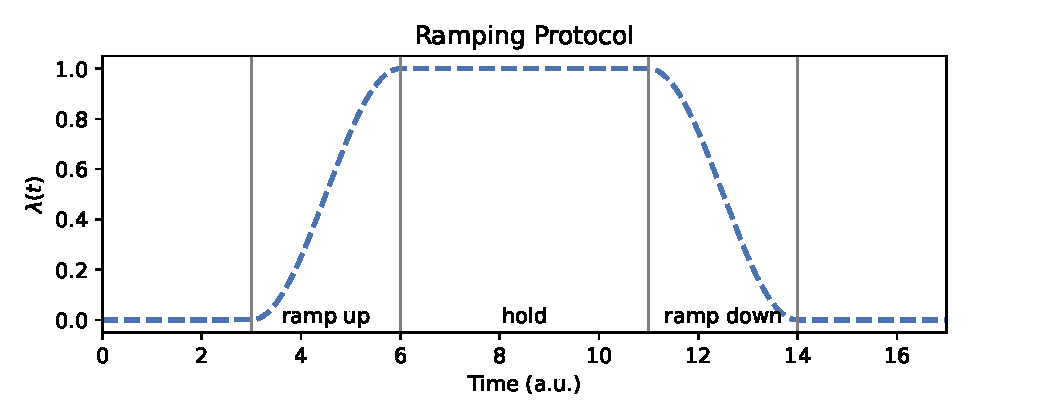
\includegraphics[width=1.0\textwidth]{figs/ramp_protocol.pdf}
    \caption{Example of a cosine ramping protocol as described in \eqref{eq:lambda_ramp}. The protocol smoothly transitions the system parameters from the initial configuration $C_I$ to the degenerate configuration $C_{II}$ and back again, allowing for controlled entanglement dynamics. The x-axis is time in atomic units (a.u), and the y-axis is the ramping parameter $\lambda(t)$, a dimensionless scalar value. In this illustration we've set $T_{\mathrm{start}} = 3$ a.u, $T_{\mathrm{up}} = 3$ a.u, $T_{\mathrm{hold}} = 5$ a.u, $T_{\mathrm{down}} = 3$ a.u, and $T_{\mathrm{end}} = 3$ a.u. This ramping protocol is symmetric, and is not necessarily optimal for our system, but shows the general structure of such a protocol.}
\end{figure}

\end{document}